\chapter{Initialisierung}

\label{ReportInitialisierung}

\section{Ausgangslage}

\section{Projektziele}

\begin{longtable}[]{@{}llc@{}}
  \toprule
  Nr.  & Zielbeschreibung                                                                       & Muss/Kann\tabularnewline
  \toprule
       & Produktziele\tabularnewline
  \midrule
  1.1  & Besucher können im Produkt nach Konzerten suchen                                       & \textbf{Muss}\tabularnewline
  1.2  & Suchresultate können nach Musik-Genre und Ort gefiltert werden                         & \textbf{Muss}\tabularnewline
  1.3  & Das Produkt soll ein modernes responsives Design vorweisen                             & \textbf{Muss}\tabularnewline
  1.4  & Konzerte sollen von Suchmaschinen indexiert werden können                              & \textbf{Muss}\tabularnewline
  1.5  & Benutzer können isch im Produkt registrieren                                           & \textbf{Muss}\tabularnewline
  1.6  & Benutzer können ihr Passwort nach Verlust neu setzen                                   & \textbf{Muss}\tabularnewline
  1.7  & Inhalte des Portals sind durch die Benutzer erfassbar und bearbeitbar                  & \textbf{Muss}\tabularnewline
  1.8  & Kompatibilität mit aktuellem Google Chrome und Mozilla Firefox Browser                 & \textbf{Muss}\tabularnewline
  1.9  & Konzerte können vom Produkt nach Facebook exportiert werden                            & Kann\tabularnewline
  1.10 & Ein angemeldeter Benutzer kann vermerken ob er einem Konzert teilnimmt                 & Kann\tabularnewline
  1.11 & Das Produkt soll sich an Security Best-Practices von OWASP halten                      & \textbf{Muss}\tabularnewline
  \bottomrule
       & Abwicklungsziele\tabularnewline
  \midrule
  2.1  & \makecell[l]{Das Projekt soll nach HERMES 5 unter Berücksichtigung der Richtlinien von                                \\ der TSBE dokumentiert werden} & \textbf{Muss}\tabularnewline
  2.2  & Das Produkt muss bis Projektende fertiggestellt und bereit für die Einführung sein     & \textbf{Muss}\tabularnewline
  2.3  & Die Technische-Umsetzung wird durch Damian Senn erstellt                               & \textbf{Muss}\tabularnewline
  2.4  & \makecell[l]{Die Kommunikation zwischen Experten und Diplomanden erfolgt wie im                                       \\ Projektauftrag \ref{kommunikation} beschrieben.} & \textbf{Muss}\tabularnewline
  2.5  & Das Projekt muss bis Ende Mai 2019 abgeschlossen sein                                  & \textbf{Muss}\tabularnewline
  \bottomrule
\end{longtable}


\clearpage

\section{Projektorganisation}

\begin{figure}[!htb]
  \centering
  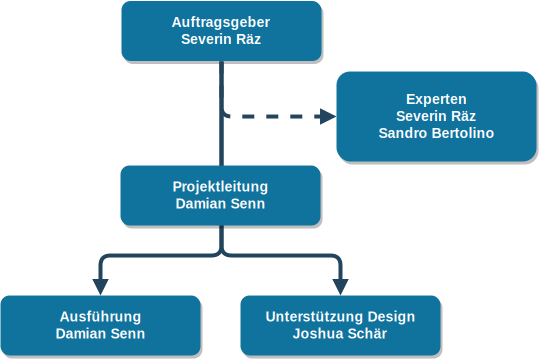
\includegraphics[width=0.8\textwidth]{figures/organigram.png}
  \caption{Organigram}
\end{figure}

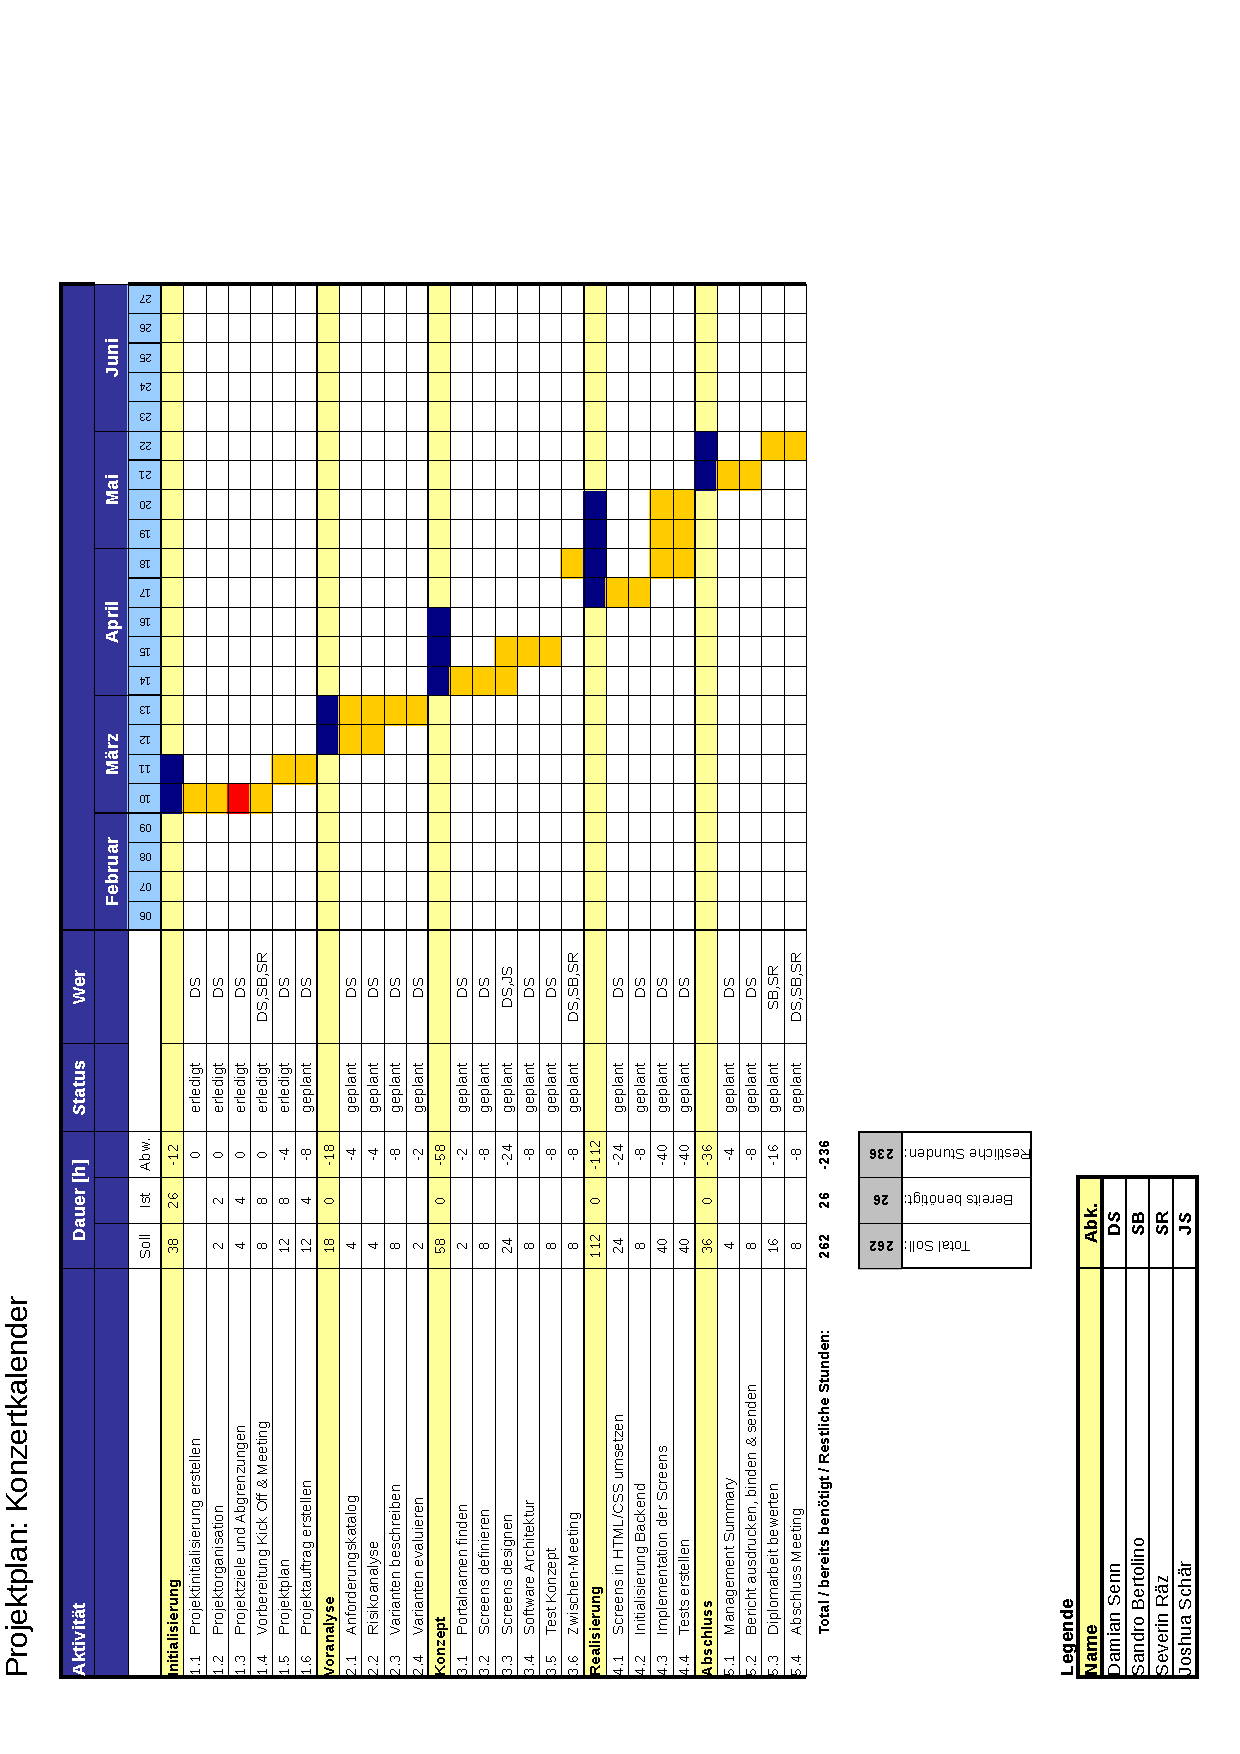
\includepdf[pagecommand={\section{Ausgefüllter Projektplan}}]{initialisierung/planung.pdf}

\section{Lieferergebnisse}

\section{Ressourcenplan}

\section{Risiken}

\clearpage

\section{Abgrenzungen}

\begin{figure}[!htb]
  \centering
  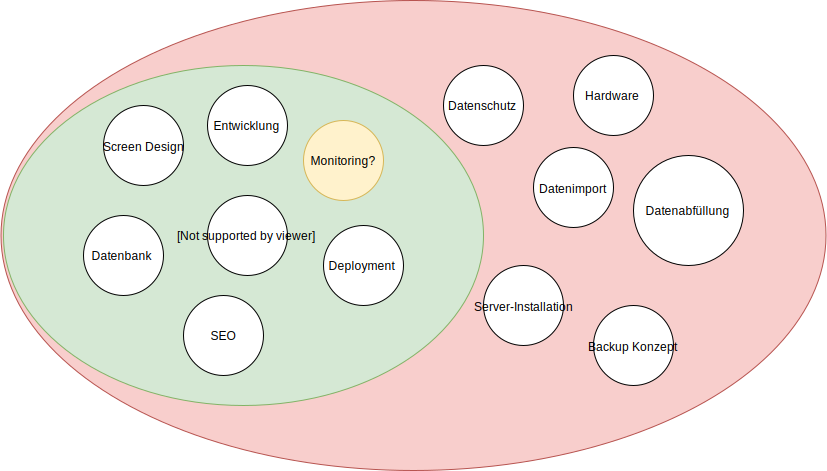
\includegraphics[width=0.95\textwidth]{figures/abgrenzungen.png}
  \caption{Abgrenzungen}
\end{figure}

Die detaillierten Erklärung zu den Abgrenzungen sind im Projektauftrag~\ref{abgrenzungen} zu finden.

\clearpage

\section{Studie}

\subsection{Informationsbeschaffung}

\clearpage
\subsection{Anforderungskatalog}

% TODO: Fix multirows across pages
%       https://tex.stackexchange.com/questions/79143/how-to-repeat-cell-content-on-next-page-for-longtable-using-multirow/79152
\begin{longtable}[]{@{}p{1.9cm}p{2.5cm}cp{5.5cm}cc@{}}
  \toprule
  \textbf{Feature}                & \textbf{Titel}             & \textbf{Nr.} & \textbf{Kriterium}                                                                                          & \textbf{Ziel} & \textbf{Muss}\tabularnewline
  \midrule
  \endhead
  \multirow{10}{*}{Suche}         & Suche nach Konzertname     & 1.1          & Listet alle Konzerte die Wörter der Suche im Konzertnamen beinhalten                                        & 1.1           & \textbf{Muss}                \\ \cline{2-6}
                                  & Suche nach Konzertlocation & 1.2          & Schränkt die Such-Resultate nach gegebener Konzertlocation ein                                              & 1.2           & \textbf{Muss}                \\ \cline{2-6}
                                  & Suche nach Ort             & 1.2          & Schränkt die Such-Resultate nach gegebenem Ort ein                                                          & 1.2           & \textbf{Muss}                \\ \cline{2-6}
                                  & Suche nach Genre           & 1.2          & Schränkt die Such-Resultate nach gegebenem Musik-Genre ein                                                  & 1.2           & \textbf{Muss}                \\
  \midrule
  \multirow{8}{*}{Design}         & Desktop                    & 2.1          & Alle Ansichten haben eine Desktop-Optimierte Variante                                                       & 1.4           & \textbf{Muss}                \\ \cline{2-6}
                                  & Tablet                     & 2.2          & Alle Ansichten haben eine Tablet-Optimierte Variante                                                        & 1.4           & \textbf{Muss}                \\ \cline{2-6}
                                  & Mobile                     & 2.3          & Alle Ansichten haben eine Mobile-Optimierte Variante                                                        & 1.4           & \textbf{Muss}                \\ \cline{2-6}
                                  & Browser Kompatibilität     & 2.4          & Alle Ansichten müssen in aktuellem Google Chrome und Mozilla Firefox dem Grundlayout folgen                 & 1.9           & \textbf{Muss}                \\
  \midrule
  \multirow{4}{*}{\acrshort{seo}} & Indexierbarkeit            & 3.1          & Das Produkt ist von Suchmaschinen indexierbar                                                               & 1.5           & \textbf{Muss}                \\ \cline{2-6}
                                  & Linked Data                & 3.2          & Konzert Detailseiten sind mit dem Event-Schema\footnote{\url{https://schema.org/MusicEvent}} ausgestattet   & 1.5           & \textbf{Muss}                \\
  \midrule
  \multirow{8}{*}{Benutzer}       & Registrierung              & 4.1          & Besucher können sich einen Benutzer registrieren, Benutzernamen und E-Mail Adressen müssen einzigartig sein & 1.6           & \textbf{Muss}                \\ \cline{2-6}
                                  & Passwort-Vergessen         & 4.2          & Benutzer können sich einen Passwort-Reset Link anfordern                                                    & 1.7           & \textbf{Muss}                \\ \cline{2-6}
                                  & Social                     & 4.3          & Benutzer können auf Konzerten vermerken ob sie Teilnehmen oder nicht                                        & 1.11          & Kann                         \\
  \midrule
  \clearpage
  \multirow{6}{*}{Erfassung}      & Artist                     & 5.1          & Benutzer können Artisten mit einem Genre erfassen                                                           & 1.8           & \textbf{Muss}                \\ \cline{2-6}
                                  & Location                   & 5.2          & Benutzer können eine Konzertlocation mit Ort/Strasse erfassen                                               & 1.8           & \textbf{Muss}                \\ \cline{2-6}
                                  & Konzert                    & 5.3          & Benutzer können ein Konzert mit Konzertlocation und Artisten erfassen                                       & 1.8           & \textbf{Muss}                \\ \cline{2-6}
                                  & Facebook                   & 5.4          & Benutzer können ein Konzert in ein Facebook-Event exportieren                                               & 1.10          & Kann                         \\
  \midrule
  \multirow{9}{*}{Security}       & SQL-Injection              & 6.1          & Das Produkt soll resistent gegen SQL-Injection sein                                                         & 1.12          & \textbf{Muss}                \\ \cline{2-6}
                                  & HTML-Injection             & 6.2          & Das Produkt soll resistent gegen HTML-Injection / \acrshort{xss} sein                                       & 1.12          & \textbf{Muss}                \\ \cline{2-6}
                                  & Passwort encryption        & 6.3          & Passwörter von Benutzer müssen mit einem sicheren Verfahren gespeichert werden                              & 1.12          & \textbf{Muss}                \\ \cline{2-6}
                                  & Session                    & 6.4          & Session-Cookies dürfen nicht durch JavaScript ausgelesen werden                                             & 1.12          & Kann                         \\
  \midrule
  Performance                     & Ladezeit                   & 7.1          & Die Seitenansichten dürfen nicht länger als 6 Sekunden auf einem 3G Netz laden                              &               & \textbf{Muss}                \\
  \midrule
  Sonstiges                       & User Tracking              & 8.1          & Benutzerverhalten soll analysiert und nachvollziehbar sein.                                                 &               & Kann                         \\
  \bottomrule
  \caption{Anforderungskatalog}
\end{longtable}


\subsection{Pflichtenheft}

\subsection{Mögliche Varianten}

\subsection{Evaluation Varianten}

\subsection{Entscheid Varianten}

\subsection{Wirtschaftlichkeit}
